% Compile with XeLaTeX or LuaLaTeX for Avenir/Avenir Next.
% In VS Code LaTeX Workshop, choose recipe: latexmk (xelatex) or lualatex.

\documentclass[aspectratio=169,11pt]{beamer}

% ------------------------------------------------------------
% Theme foundation
% ------------------------------------------------------------
\usetheme{Antibes}
\useoutertheme{miniframes}      % top progress circles
\useinnertheme{rectangles}
\setbeamertemplate{navigation symbols}{} % no navigation icons near footer

% ------------------------------------------------------------
% Font setup: Avenir if available, graceful fallback otherwise
% ------------------------------------------------------------
\usepackage{iftex}
\ifPDFTeX
  % Fallback for accidental pdfLaTeX compilation.
  % For the intended look, compile with XeLaTeX or LuaLaTeX.
  \usepackage[T1]{fontenc}
  \usepackage[utf8]{inputenc}
  \usepackage{helvet}
  \renewcommand{\familydefault}{\sfdefault}
\else
  \usepackage{fontspec}
  \IfFontExistsTF{Avenir Next}{%
    \setsansfont{Avenir Next}[
      UprightFont = *,
      BoldFont = * Demi Bold,
      ItalicFont = * Italic,
      BoldItalicFont = * Demi Bold Italic
    ]
  }{%
    \IfFontExistsTF{Avenir}{%
      \setsansfont{Avenir}
    }{%
      % TeX Live fallback with a similar clean sans feel.
      \setsansfont{TeX Gyre Heros}
    }%
  }%
  \renewcommand{\familydefault}{\sfdefault}
\fi

% Keep math in a traditional serif math font for readability.
\usefonttheme{professionalfonts}
\usefonttheme[onlymath]{serif}


% ------------------------------------------------------------
% Packages
% ------------------------------------------------------------
\usepackage{amsmath,amssymb,mathtools}
\usepackage{graphicx}
\usepackage{xcolor}
\usepackage{tikz}
\usepackage{hyperref}
\usetikzlibrary{calc}

% ------------------------------------------------------------
% Color palette
% ------------------------------------------------------------
\definecolor{TwilightIvory}{HTML}{F6F1EA}
\definecolor{TwilightIvorySoft}{HTML}{FBF8F3}
\definecolor{TwilightCarbon}{HTML}{111111}
\definecolor{TwilightBlack}{HTML}{080808}
\definecolor{TwilightInk}{HTML}{050506}

\definecolor{TwilightDarkViolet}{HTML}{1E1533}
\definecolor{TwilightPurple}{HTML}{43305C}
\definecolor{TwilightPlum}{HTML}{2A1A42}
\definecolor{TwilightMulberry}{HTML}{7A4A63}

\definecolor{TwilightDeepTeal}{HTML}{0D7C7B}
\definecolor{TwilightAqua}{HTML}{A8E5DA}
\definecolor{TwilightBlush}{HTML}{F0D2DF}
\definecolor{TwilightRose}{HTML}{D8A4BF}

% ------------------------------------------------------------
% Global colors
% ------------------------------------------------------------
\setbeamercolor{normal text}{fg=TwilightCarbon,bg=TwilightIvory}
\setbeamercolor{background canvas}{bg=TwilightIvory}
\setbeamercolor{structure}{fg=TwilightDeepTeal}
\setbeamercolor{alerted text}{fg=TwilightMulberry}
\setbeamercolor{example text}{fg=TwilightDeepTeal}

\setbeamercolor{title}{fg=TwilightDarkViolet,bg=TwilightIvory}
\setbeamercolor{subtitle}{fg=TwilightPurple,bg=TwilightIvory}
\setbeamercolor{author}{fg=TwilightDeepTeal,bg=TwilightIvory}
\setbeamercolor{institute}{fg=TwilightCarbon,bg=TwilightIvory}
\setbeamercolor{date}{fg=TwilightCarbon,bg=TwilightIvory}

\setbeamercolor{frametitle}{fg=TwilightIvory,bg=TwilightDarkViolet}
\setbeamercolor{framesubtitle}{fg=TwilightAqua,bg=TwilightDarkViolet}

% ------------------------------------------------------------
% Title Slide Image
% ------------------------------------------------------------

% ------------------------------------------------------------
% Header bars: black, dark violet, purple descending from top
% ------------------------------------------------------------
\setbeamercolor{headline top}{fg=TwilightIvory,bg=TwilightBlack}
\setbeamercolor{headline middle}{fg=TwilightAqua,bg=TwilightDarkViolet}
\setbeamercolor{headline bottom}{fg=TwilightBlush,bg=TwilightPurple}

\setbeamercolor{section in head/foot}{fg=TwilightIvory,bg=TwilightBlack}
\setbeamercolor{subsection in head/foot}{fg=TwilightAqua,bg=TwilightDarkViolet}
\setbeamercolor{section in head/foot shaded}{fg=TwilightIvory!45!TwilightBlack,bg=TwilightBlack}
\setbeamercolor{subsection in head/foot shaded}{fg=TwilightBlush,bg=TwilightDarkViolet}



% Custom three-bar headline.  The bottom bar carries the miniframe progress meter.
\setbeamertemplate{headline}{%
  \leavevmode%
  \begin{beamercolorbox}[wd=\paperwidth,ht=2.25ex,dp=.75ex,leftskip=1.1em,rightskip=1.1em]{headline top}%
    \usebeamerfont{section in head/foot}
    \progressbar

  \end{beamercolorbox}%
  \begin{beamercolorbox}[wd=\paperwidth,ht=2.15ex,dp=.65ex,leftskip=1.1em,rightskip=1.1em]{headline middle}%
    \usebeamerfont{subsection in head/foot}\insertsubsectionnavigationhorizontal{\paperwidth}{}{}%
  \end{beamercolorbox}%
  \begin{beamercolorbox}[wd=\paperwidth,ht=2.05ex,dp=.6ex,leftskip=1.1em,rightskip=1.1em]{headline bottom}%
    \insertnavigation{\paperwidth}%
  \end{beamercolorbox}%
}

% ------------------------------------------------------------
% Footer: light cream/aqua/pink text, no navigation symbols
% ------------------------------------------------------------
\setbeamercolor{footline title}{fg=TwilightIvory,bg=TwilightBlack}
\setbeamercolor{footline author}{fg=TwilightAqua,bg=TwilightBlack}
\setbeamercolor{footline page}{fg=TwilightIvory,bg=TwilightBlack}

\setbeamertemplate{footline}{%
  \leavevmode%
  \hbox{%
    \begin{beamercolorbox}[wd=.46\paperwidth,ht=2.7ex,dp=1ex,leftskip=1em]{footline title}%
      \usebeamerfont{footline}\insertshorttitle
    \end{beamercolorbox}%
    \begin{beamercolorbox}[wd=.34\paperwidth,ht=2.7ex,dp=1ex,leftskip=.5em]{footline author}%
      \usebeamerfont{footline}\insertshortauthor
    \end{beamercolorbox}%
    \begin{beamercolorbox}[wd=.20\paperwidth,ht=2.7ex,dp=1ex,rightskip=1em plus1fil]{footline page}%
      \usebeamerfont{footline}\hfill\insertframenumber{} / \inserttotalframenumber
    \end{beamercolorbox}%
  }%
}

% ------------------------------------------------------------
% Blocks
% ------------------------------------------------------------
\setbeamercolor{block title}{fg=TwilightIvory,bg=TwilightDarkViolet}
\setbeamercolor{block body}{fg=TwilightCarbon,bg=TwilightIvorySoft}

\setbeamercolor{block title alerted}{fg=TwilightIvory,bg=TwilightMulberry}
\setbeamercolor{block body alerted}{fg=TwilightCarbon,bg=TwilightBlush!28!TwilightIvorySoft}

\setbeamercolor{block title example}{fg=TwilightIvory,bg=TwilightDeepTeal}
\setbeamercolor{block body example}{fg=TwilightCarbon,bg=TwilightAqua!20!TwilightIvorySoft}

% ------------------------------------------------------------
% Typography and spacing
% ------------------------------------------------------------
\setbeamerfont{title}{size=\LARGE,series=\bfseries}
\setbeamerfont{subtitle}{size=\large,series=\mdseries}
\setbeamerfont{author}{size=\normalsize,series=\mdseries}
\setbeamerfont{frametitle}{size=\Large,series=\bfseries}
\setbeamerfont{framesubtitle}{size=\normalsize,series=\mdseries}
\setbeamerfont{section in head/foot}{size=\scriptsize,series=\bfseries}
\setbeamerfont{subsection in head/foot}{size=\scriptsize,series=\mdseries}
\setbeamerfont{footline}{size=\scriptsize,series=\mdseries}
\setbeamerfont{block title}{series=\bfseries}

\setbeamersize{text margin left=1.15em,text margin right=1.15em}
\setlength{\parskip}{0.35em}

% ------------------------------------------------------------
% Bullets and links
% ------------------------------------------------------------
\setbeamercolor{item}{fg=TwilightDeepTeal}
\setbeamercolor{subitem}{fg=TwilightPurple}
\setbeamercolor{subsubitem}{fg=TwilightMulberry}
\setbeamertemplate{itemize item}{\raise0.2ex\hbox{\scriptsize$\blacktriangleright$}}
\setbeamertemplate{itemize subitem}{\raise0.15ex\hbox{\tiny$\blacktriangleright$}}

\setbeamercolor{progress active}{fg=TwilightMulberry}
\setbeamercolor{progress inactive}{fg=TwilightIvory}
\setbeamercolor{progress complete}{fg=TwilightDarkTeal}


% ------------------------------------------------------------
% Document Specific Data
% ------------------------------------------------------------
\title[ML FEM]{Multilevel Methods on Finite Elements}
\author[MB \& NK]{Melayne Barker and Neal Kuperman\\ Panayot Vassilevski}
\institute{Portland State University}
\date{\today}
\definecolor{myactive}{HTML}{7A4A63} 
\definecolor{mycomplete}{HTML}{0D7C7B}
\definecolor{myinactive}{HTML}{F6F1EA}
\newcounter{progresssteps}
\setcounter{progresssteps}{13} % number of hats

\newcommand{\progressbar}{
\begin{tikzpicture}[remember picture,overlay]
    \foreach \i in {1,...,13} {
        % position along top
        \pgfmathsetmacro{\x}{(\i-1)*1.0}

        % determine if this hat should be active
        \pgfmathparse{\insertframenumber/\inserttotalframenumber*14 >= \i}
        \ifnum\pgfmathresult<1
            \colorlet{hatcolor}{myactive}
        \else
          \ifnum\pgfmathresult>1
            \colorlet{hatcolor}{myinactive}
          \else
            \colorlet{hatcolor}{mycomplete}
          \fi
        \fi

        % hat function
        \draw[fill=hatcolor,draw=hatcolor,fill opacity=0.25]
            ($(current page.north west)+(0.8+\x,-0.3)$)
            -- ++(0.35,0.25)
            -- ++(0.35,-0.25)
            -- cycle;
    }
\end{tikzpicture}
}
\begin{document}
\begin{centering}
\begin{frame}
  \titlepage
  \begin{tikzpicture}[remember picture, overlay]
    \node[
      anchor=south,
      inner sep=0pt
    ] at (current page.south) {
      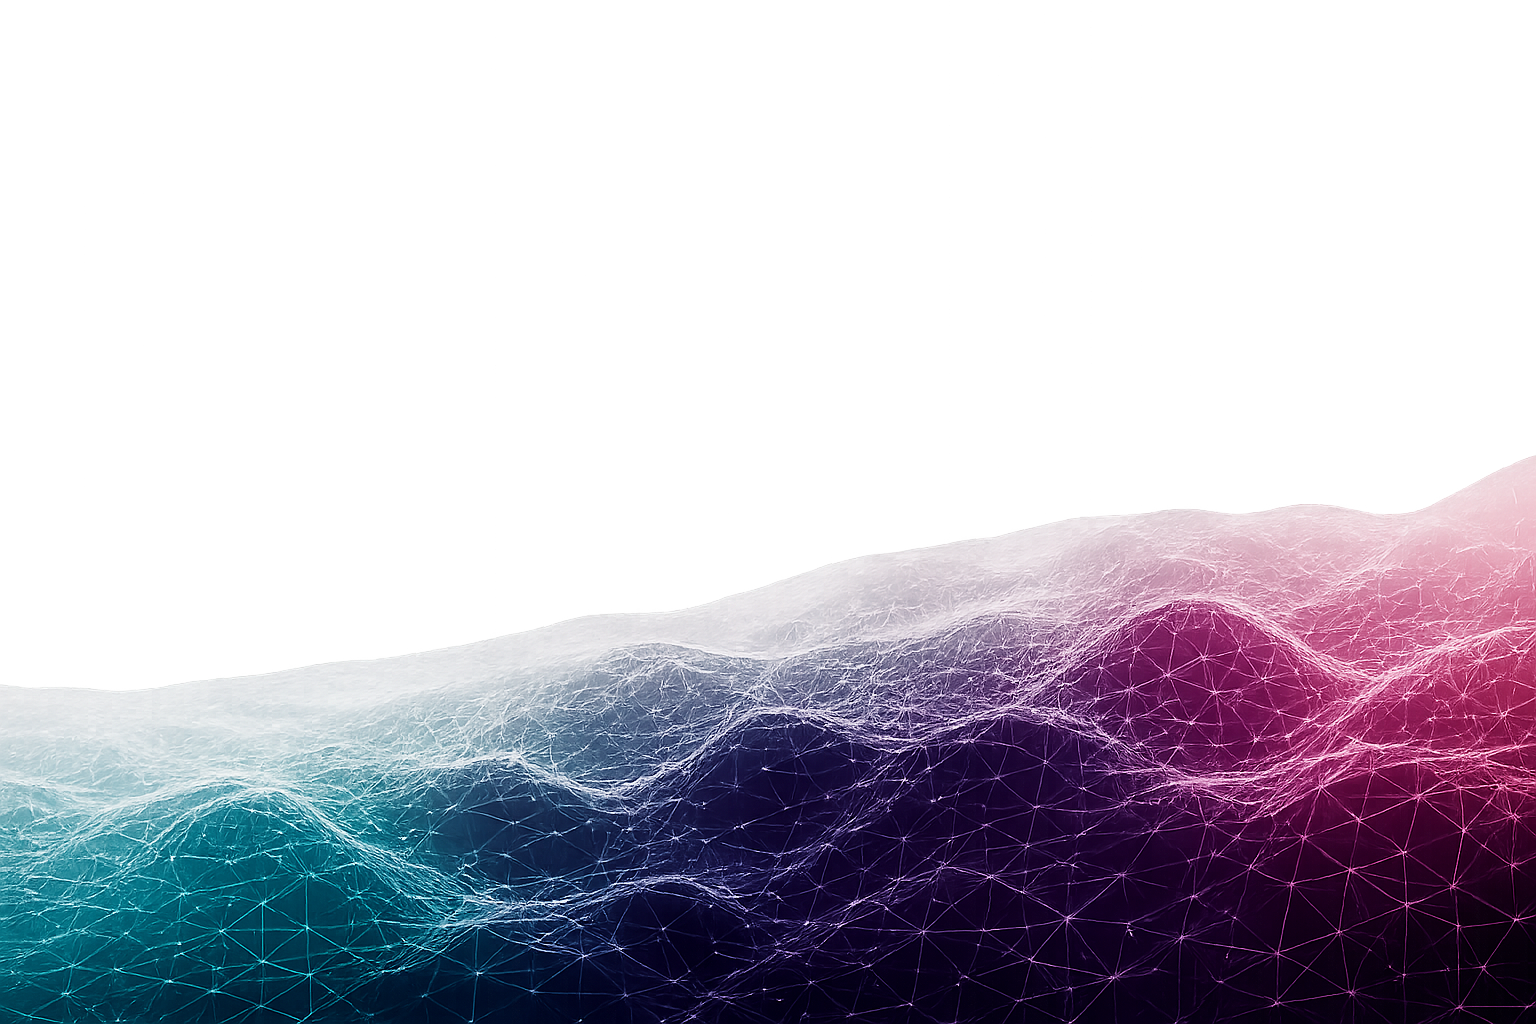
\includegraphics[
        width=\paperwidth,
        height=0.64\paperheight
      ]{images/fem_title_graphic.png}
    };
  \end{tikzpicture}
\end{frame}

\section{The Problem}
\begin{frame}{Modeling subsurface flow}
  \begin{alert}{The Idea}
    Implement Multilevel Monte Carlo for subsurface flow via random coefficients. First stage was to implement a multilevel solver in NGSolve that could handle variable coefficients.
  \end{alert}

  We use \( H_1 \)-conforming piecewise linear finite elements applied to the Poisson problem with variable coefficients and Dirichlet boundary conditions on the unit square.
  \begin{align*}
    K\left(x,y\right) = 1 + x^2 + y^2\\
    \sigma = 0.5\\
    K\left(x,y\right)\Delta u+ \sigma^2 u = 0\\
    \Omega = \left[0,1\right]\times\left[0,1\right]
  \end{align*}
  On the left side, \( u(0,y) = 1 \), on the rest of the boundary \( u(x,y)_{\partial \Omega} = 0 \).
\end{frame}


\section{The Approach}
\begin{frame}{NGSolve}
  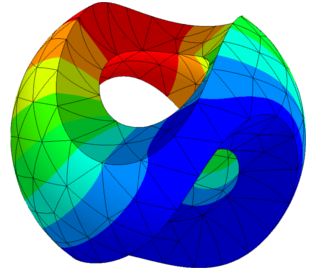
\includegraphics[
      height=0.150\textheight
    ]{images/logo1.png}
  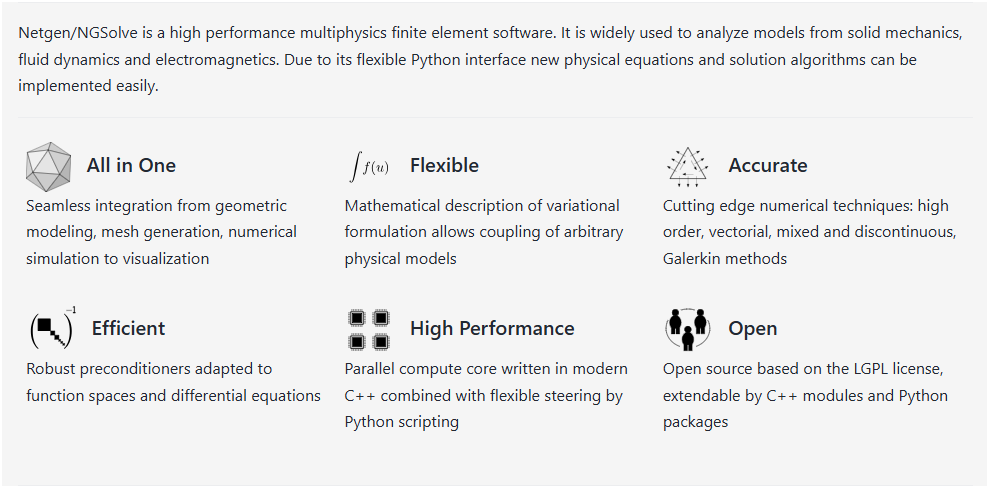
\includegraphics[
      height=0.750\textheight
    ]{images/ngsolve.png}
\end{frame}

\begin{frame}{Really Big Problems}
    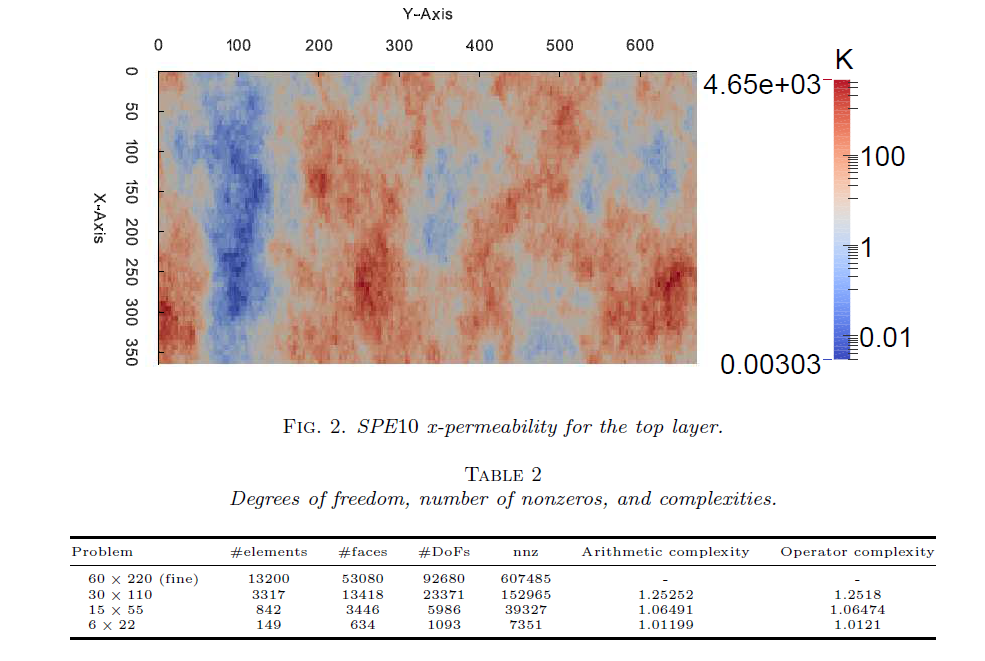
\includegraphics[
      height=.9\textheight
    ]{images/fluidspread.png}
\end{frame}

\section{Our Methods}

\subsection{Our Constructed Framework}
\begin{frame}{A Hierarchy of Finite Element Spaces}
   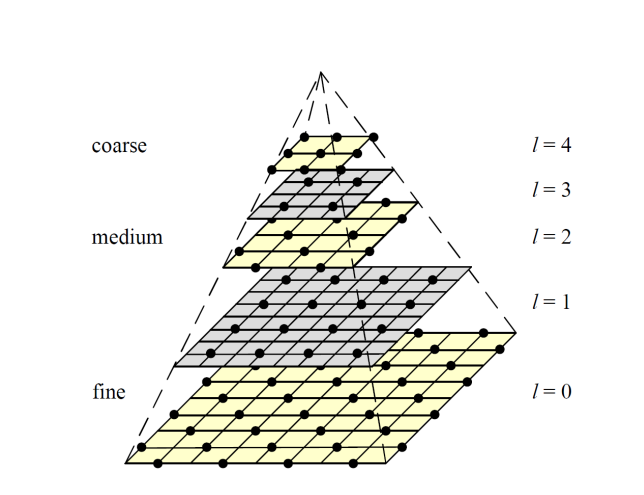
\includegraphics[
      height=0.750\textheight
    ]{images/multigrid.png}
\end{frame}

\begin{frame}{Setting up the finite element spaces}
  At each level, we have the data storage, solving tools, and projection matrices available.
  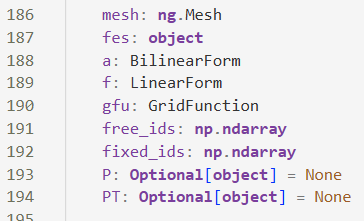
\includegraphics[
    height=0.75\textheight
  ]{images/level-parts.png}
\end{frame}



\begin{frame}{Solving V-cycle with smoothing and coarse solve}
  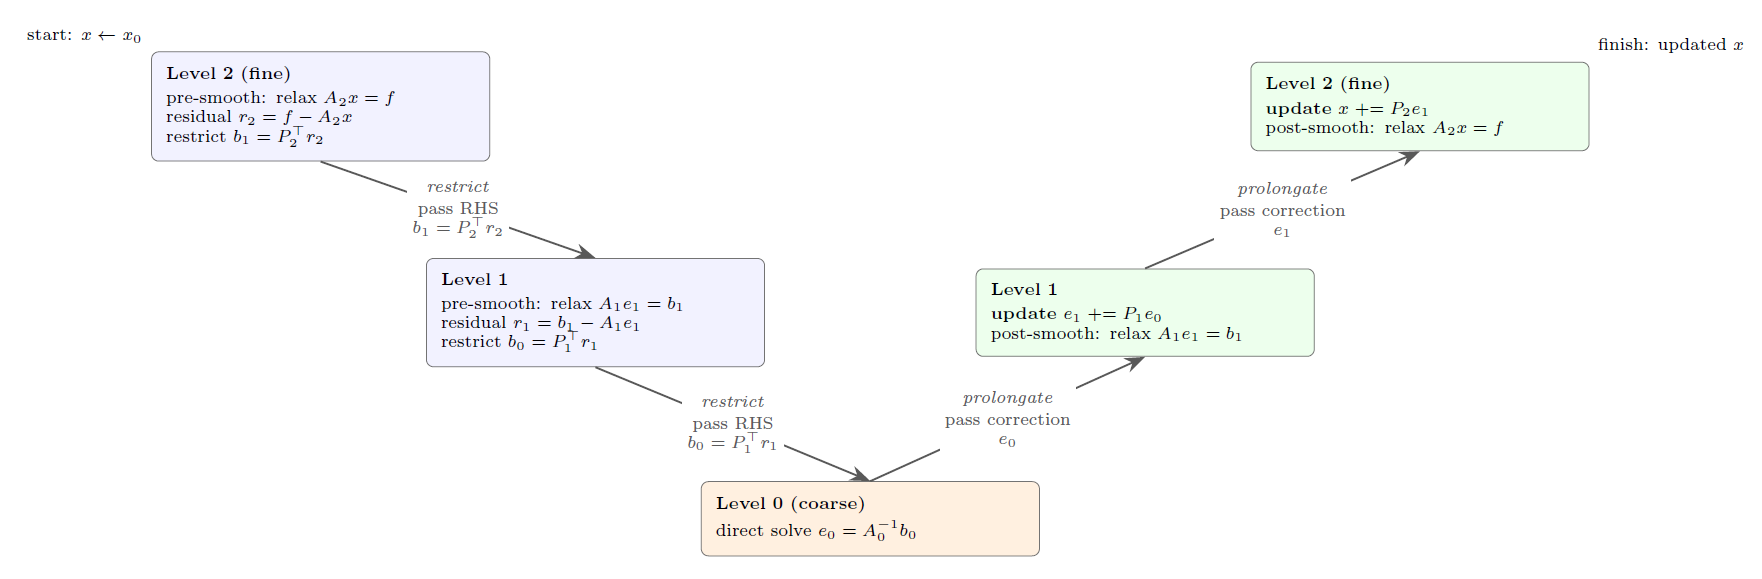
\includegraphics[
          width=\textwidth
        ]{images/vcycle.png}
\end{frame}

\section{Our Results}
\begin{frame}{Initial Iterate}
    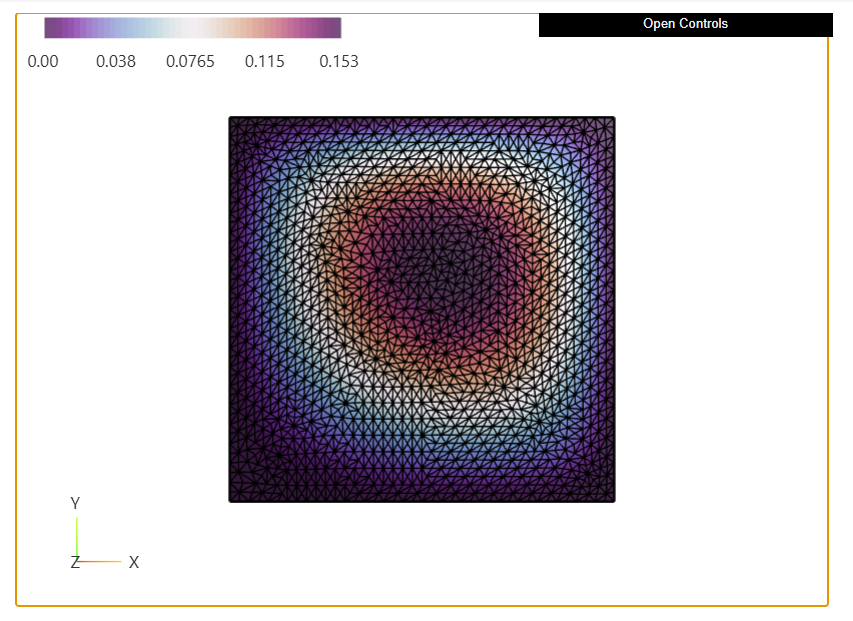
\includegraphics[
          height=.8\textheight
        ]{images/smooth1.png}

    fine ndof=1961, coarse ndof=511,  $P$ shape 1961x511
\end{frame}

\begin{frame}{Gauss Seidel Smoothing}
    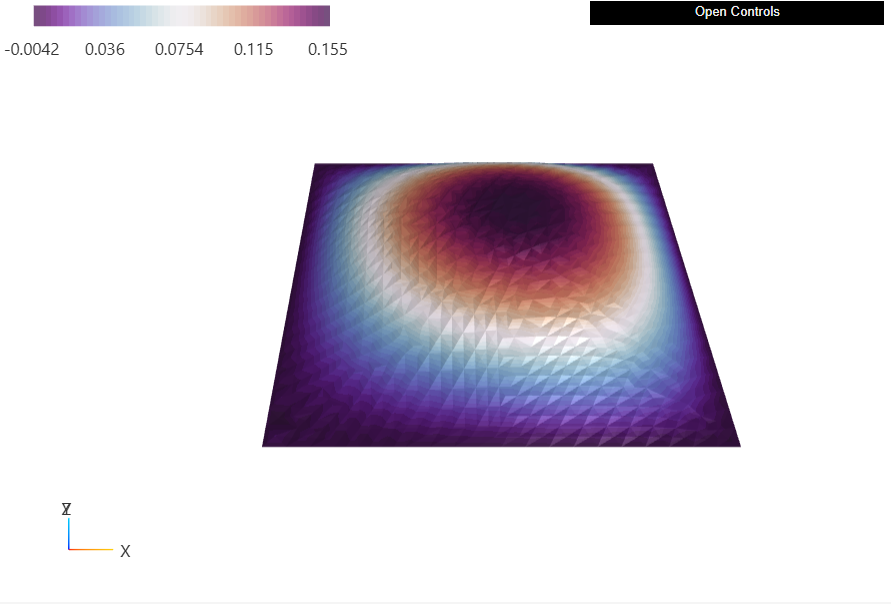
\includegraphics[
          height=.75\textheight
        ]{images/smooth2.png}

    $\left\| e \right\|_E $ (after section 1 pre-smooth): 1.790578\\
    $\left\| e \right\|$ L2 error:       9.820784e-04
\end{frame}

\begin{frame}{Example with more layers}
  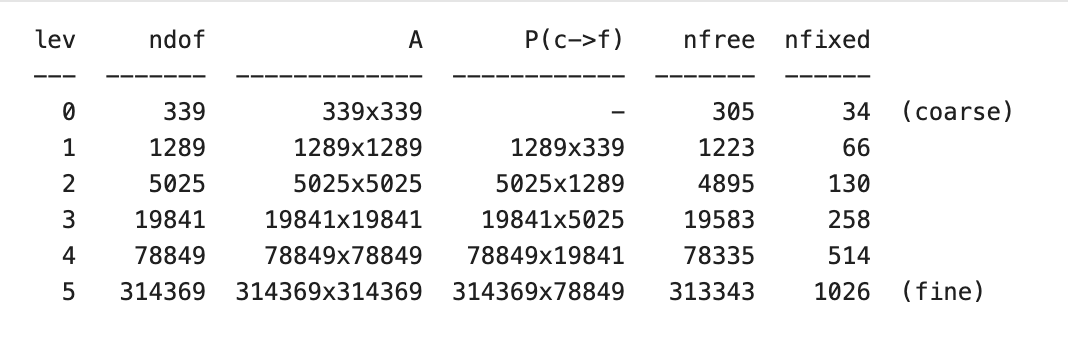
\includegraphics[width=.9\textwidth]{images/hierarchysizes.png}
\end{frame}

\begin{frame}{Compare to CG}
  \begin{alert}{Success!}
  We made it so that we run PCG and when it asks for a preconditioner, it gets our two-level method
  \end{alert}
  
  PCG (NGSolve CG + V-cycle): 1684 iterations
   
  In contrast, we compared Conjugate Gradient on meshes of different sizes to see how the convergence varies.

  \begin{tabular}{|c|c|c|c|}
    \hline
    Total DoFs & CG Iterations & Initial Residual & Final Residual\\
    \hline
    339 & 71 & 4.074 & \( 3.13 \times 10^{-10} \)\\
    1,289 & 182 & 3.1133 & \( 2.78 \times 10^{-10} \)\\
    5,025 & 364 & 1.637 & \( 1.60 \times 10^{-10} \)\\
    19,841 & DNC & 0.869 & \( 9.6 \times 10^{-7} \)\\
    78,849 & DNC & 0.478 & \( 1.56 \times 10^{-3} \) \\
    314,369 & DNC & 0.277 & \( 9.92 \times 10^{-2} \)\\
    \hline
  \end{tabular}

\end{frame}

\section{Conclusion}
\begin{frame}{Conclusion}
  \begin{itemize}
    \item We demonstrated the smoothing effects of Gauss Seidel on highly oscillatory components.
    \item We implemented a two-level method with GS smoothing and a coarse direct solve.
    \item We built a framework from which future multilevel test on NGSolve finite element spaces may be performed and tested it to demonstrate convergence.
    \item We implemented the method above as the preconditioner for a preconditioned conjugate gradient solver.
    \item After the work here, we implemented fully random coefficients using a Karhunen-Lo\`{e}ve expansion. (Spoilers)
  \end{itemize}
\end{frame}
\end{centering}

\section{References}
\begin{frame}
  \begin{itemize}
    \item M. la Cour Christensen, U. Villa, A. P. Engsig-Karup, and P. S. Vassilevski, "Numerical Multilevel Upscaling for Incompressible Flow in Reservoir Simulation: An Element-Based Algebraic Multigrid (AMGe) Approach," SIAM J. Sci. Comput., vol. 39, no. 1, pp. B102–B137, 2017.
    \item P. S. Vassilevski, "Multilevel Block Factorization Preconditioners, Matrix-based Analysis and Algorithms for Solving Finite Element Equations", Springer, New York, 2008.
    \item J. S. Ovall, Numerical Mathematics. Philadelphia, PA: SIAM, 2024. 
    \item J. N. Reddy, N. K. Anand, and P. Roy, Finite Element and Finite Volume Methods for Heat Transfer and Fluid Dynamics. Cambridge University Press, Cambridge, UK, 2023. 
    \item Schöberl, J., et al. NGSolve Interactive Tutorials (i-Tutorials). Netgen/NGSolve Documentation. 
    \item Dilip Krishnan, Richard Szeliski "Multigrid and Multilevel Preconditioners for Computational Photography" 
  \end{itemize}
\end{frame}
\end{document}
